\documentclass{lecture}

\usepackage{pgf-pie}

\institute{Institut für Statistik und Wirtschaftsmathematik}
\title{Vorlesung 2}
\author{Joshua Feld, 406718}
\course{Statistik}
\professor{Cramer}
\semester{Sommersemester 2022}
\program{CES (Bachelor)}

\begin{document}
    \maketitle


    Ein Merkmal wird als qualitativ bezeichnet, wenn die zugehörigen Merkmalsausprägungen nur eine Zugehörigkeit oder eine Beurteilung wiedergeben.
    Das Merkmal dient in diesem Fall zur Unterscheidung verschiedener Arten von Eigenschaften.
    Die Zugehörigkeiten werden dabei häufig entweder durch Namen oder durch die Zuordnung von Ziffern beschrieben.

    \begin{example}
        In der Schule werden sechs Noten zur Bewertung verwendet: sehr gut, gut, befriedigend, ausreichend, mangelhaft, ungenügend.
        Schulnoten sind damit qualitative Merkmale.
        Meist werden statt der konkreten Bezeichnungen für die Schulnoten jedoch nur die Zahlen zwischen eins und sechs angegeben.
        Aber selbst wenn den Noten die Zahlen \(1, \ldots, 6\) zugeordnet werden, bleibt das Merkmal \emph{Note} qualitativer Natur, die Zahlen dienen lediglich der kurzen Notation.
        Wesentlich zur Unterscheidung zum quantitativen Merkmal ist, dass die Notendifferenzen keine Bedeutung im Sinne eines Messwerts haben (Ist der Abstand zwischen den Noten \(1\) und \(2\) genauso groß wie der zwischen den Noten \(5\) und \(6\)?).
    \end{example}

    Qualitative Merkmale, deren Ausprägungen lediglich durch Begriffe (Namen) beschrieben werden, heißen nominalskaliert oder auch nominale Merkmale.
    Auf einer Skala werden die Ausprägungen dabei im Allgemeinen mit Zahlen kodiert.
    Die Ausprägungen eines nominalen Merkmals können lediglich hinsichtlich ihrer Gleichheit (Ungleichheit) verglichen werden.
    Eine Reihung (Ordnung) der Ausprägungen ist, auch wenn diese in Form von Zahlen angegeben werden, nicht möglich oder nicht sinnvoll.
    Ergebnisse von Rechnungen mit diesen Zahlenwerten sind i.A. nicht interpretierbar.
    Kann ein nominales Merkmal nur zwei mögliche Ausprägungen (z.B. ja/nein, intakt/defekt, \(0\)/\(1\)) annehmen, so wird speziell von einem dichotomen Merkmal gesprochen.

    \begin{example}
        \begin{enumerate}
            \item Das Merkmal \emph{Familienstand} einer Person ist nominalskaliert.
            Die möglichen Merkmalsausprägungen \emph{ledig}, \emph{verheiratet}, \emph{verwitwet} und \emph{geschieden} sind nur hinsichtlich ihrer Gleichheit/Verschiedenheit vergleichbar.
            Auch die Vergabe der Ziffern \(1, \ldots, 4\) an die verschiedenen Merkmalsausprägungen, wie z.B. in der Datenerfassung mit Fragebögen üblich, würde daran nichts ändern.
            Weitere personenbezogene nominale Merkmale sind z.B. Geschlecht, Haarfarbe, Augenfarbe oder Religionszugehörigkeit.
            \item In einem Großunternehmen wird bei einer Bewerbung die Teilnahme an einem schriftlichen Einstellungstest vorausgesetzt.
            Das darin erzielte Ergebnis entscheidet über die Einladung zu einem persönlichen Gespräch.
            Abhängig vom Grad der erfolgreichen Bearbeitung der gestellten Aufgaben gilt der Test als \emph{bestanden} oder \emph{nicht bestanden}.
            Das Ergebnis des Einstellungstests ist daher ein dichotomes Merkmal.
        \end{enumerate}
    \end{example}

    Qualitative Merkmale, deren Ausprägungen einer Rangfolge genügen, heißen ordinalskaliert oder ordinale Merkmale.
    Die Ausprägungen eines ordinalskalierten Merkmals sind hinsichtlich ihrer Größe vergleichbar, d.h. es kann jeweils unterschieden werden, ob eine Ausprägung kleiner, gleich oder größer (bzw. schlechter, gleich oder besser) einer anderen ist.
    Auf einer Skala werden (wie bei nominalen Merkmalen) meist ganze Zahlen zur Kodierung verwendet.
    Da den Abständen zwischen unterschiedlichen Ausprägungen eines ordinalen Merkmals allerdings in der Regel keine Bedeutung zukommt, sind Rechnungen mit diesen Zahlen ebenfalls i.A. nicht sinnvoll.

    \begin{example}
        Eine Schulnote ist ein Merkmal mit den Ausprägungen \emph{sehr gut}, \emph{gut}, \emph{befriedigend}, \emph{ausreichend}, \emph{mangelhaft} und \emph{ungenügend}.
        Schulnoten stellen ordinale Merkmale dar.
        Den Ausprägungen werden in Deutschland meist die Zahlenwerte \(1, \ldots, 6\) zugeordnet.
        Ebenso könnten stattdessen aber auch die Zahlen \(1, 11, 12, 13, 14, 24\) verwendet werden, um zu verdeutlichen, dass die beste und die schlechteste Note eine besondere Rolle spielen.
        Damit wird klar, dass sich der Abstand zwischen einzelnen Noten nicht sinnvoll interpretieren lässt.
        Im amerikanischen Bewertungsschema wird dies dadurch deutlich, dass die Güte einer Note durch die Stellung des zugehörigen Buchstabens (\(A, B, C, D, E, F\)) im Alphabet wiedergegeben wird.
        Dies unterstreicht insbesondere, dass Abstände zwischen Noten in der Regel nicht quantifizierbar sind.
    \end{example}

    \begin{example}
        Die Berechnung von Durchschnittsnoten ist eine übliche Vorgehensweise, wobei die Rechenoperation zur Bildung eines solchen Notenmittelwerts ein Ergebnis haben kann, das als Note selbst nicht vorkommt (z.B. \(2,5\)).
        Da den Abständen zwischen Noten keine Bedeutung zugeordnet werden kann, ist ein solches Ergebnis nicht ohne Weiteres interpretierbar.
        Trotzdem kommt diesem Vorgehen sehr wohl eine sinnvolle Bedeutung zu.
        Die Durchschnittsnote kann zum Vergleich der Gesamtleistungen herangezogen werden.
        Dieser Vergleich ist aber natürlich nur dann zulässig, wenn davon ausgegangen werden kann, dass die Einzelnoten unter vergleichbaren äußeren Umständen (Bewertung von Leistungen in einer Klausur, Klasse, etc.) vergeben wurden -- und die Abstände zwischen aufeinander folgenden Noten als gleich angesehen werden.
    \end{example}

    Ein Merkmal wird als quantitativ bezeichnet, wenn die möglichen Merkmalsausprägungen sich durch Zahlen erfassen lassen und die Abstände (Differenzen) zwischen diesen Zahlen sinnvoll interpretierbar sind.
    Aus diesem Grund werden quantitative Merkmale auch metrisch (metrischskaliert) genannt.

    \begin{example}
        \begin{enumerate}
            \item In einer Firma zur Herstellung von Bekleidungsartikeln wird der Umsatz analysiert.
            Dabei werden u.a. auch die Anzahl der verkauften Pullover und der Wert aller verkauften Hemden ermittelt.
            Beide Merkmale sind metrisch, da Differenzen dieser Ausprägungen (in diesem Fall z.B. beim Vergleich der Verkaufszahlen mit denjenigen aus dem Vorjahr) interpretierbare Ergebnisse liefern (z.B. Umsatzzugewinn oder -rückgang).
            \item In einer Stadt wird einmal pro Tag an einer Messeinrichtung die Temperatur gemessen.
            Dieses Merkmal ist metrisch, denn Differenzen von Temperaturen lassen sich als Temperaturunterschiede sinnvoll interpretieren.
        \end{enumerate}
    \end{example}

    Quantitative Merkmale können auf zweierlei Weise unterschieden werden.
    Eine Einteilung auf der Basis von Eigenschaften der Merkmalsausprägungen führt zu intervallskalierten, verhältnisskalierten und absolutskalierten Merkmalen.
    Ein Vergleich der Anzahl von möglichen Merkmalsausprägungen liefert eine Trennung in diskrete und stetige Merkmale.

    Ein intervallskaliertes Merkmal muss lediglich die definierenden Eigenschaften eines quantitativen Merkmals erfüllen.
    Insbesondere müssen die Abstände der Ausprägungen eines intervallskalierten Merkmals sinnvoll interpretierbar sein.
    Definitionsgemäß ist daher  jedes quantitative Merkmal intervallskaliert.
    Der Begriff dient lediglich zur Abgrenzung gegenüber Merkmalen, deren Ausprägungen zusätzlich weitere Eigenschaften aufweisen.
    Es ist wichtig zu betonen, dass die Skalen, die zur Messung eines intervallskalierten Merkmals verwendet werden, keinen natürlichen Nullpunkt besitzen müssen.

    \begin{example}
        Im Beispiel 10 (Temperaturskala) aus der ersten Vorlesung wird deutlich, dass die verschiedenen Skalen unterschiedliche Nullpunkte besitzen.
        Die zugehörigen Werte sind in der folgenden Tabelle aufgeführt.
        \begin{center}
            \begin{tabular}{cccc}
                \toprule
                Nullpunkt & \si{\degreeCelsius} & \si{\degreeFahrenheit} & \si{\kelvin}\\
                \midrule
                \(0\si{\degreeCelsius}\) & \(0\) & \(32\) & \(273\)\\
                \(0\si{\degreeFahrenheit}\) & \(-17,78\) & \(0\) & \(255,22\)\\
                \(0\sis{\kelvin}\) & \(-273\) & \(-459,4\) & \(0\)\\
                \bottomrule
            \end{tabular}
        \end{center}
    \end{example}

    \begin{example}
        Mittels eines Kalenders kann die Zeit in Tage, Wochen, Monate, und Jahre eingeteilt werden.
        Die Abstände zwischen je zwei Zeitpunkten können damit sinnvoll als Zeiträume interpretiert werden.
        Die Zeit ist also ein intervallskaliertes Merkmal.
        Der Beginn der Zeitrechnung, d.h. der Nullpunkt der Skala, kann jedoch unterschiedlich gewählt werden.
        So entspricht z.B. der Beginn der Jahreszählung im jüdischen Kalender dem Jahr 3761 v.Chr. unserer Zeitrechnung (dem gregorianischen Kalender).
    \end{example}

    Ein quantitatives Merkmal heißt verhältnisskaliert, wenn die zur Messung verwendeten Skalen einen gemeinsamen natürlichen Nullpunkt aufweisen.
    Verhältnissen (Quotienten) von Merkmalsausprägungen eines verhältnisskalierten Merkmals kann eine sinnvolle Bedeutung zugeordnet werden.
    Der natürliche Nullpunkt garantiert nämlich, dass Verhältnisse von einander entsprechenden Ausprägungen, die auf unterschiedlichen (linearen) Skalen (d.h. in anderen Maßeinheiten) gemessen wurden, immer gleich sind.
    Verhältnisskalierte Merkmale sind ein Spezialfall von intervallskalierten Merkmalen.

    \begin{example}
        \begin{enumerate}
            \item Für einen Bericht in einer Motorsportzeitschrift werden die Höchstgeschwindigkeiten von Sportwagen ermittelt.
            Das Merkmal \emph{Höchstgeschwindigkeit} eines Fahrzeugs ist verhältnisskaliert.
            Unabhängig davon, ob die Geschwindigkeit in \si{\kilo\meter\per\hour} oder \si{\meter\per\second} gemessen wird (\(1\sis{\kilo\meter\per\hour} = \frac{1}{3,6}\sis{\meter\per\second}\)), bleibt der Nullpunkt der Skalen immer gleich.
            Er entspricht dem Zustand ``keine Bewegung''.
            \item Für eine Umsatzanalyse in einem Unternehmen wird jährlich der Gesamtwert aller verkauften Produkte bestimmt.
            Dieses Merkmal ist verhältnisskaliert, denn bei der Messung des Gesamtwerts gibt es nur einen sinnvollen Nullpunkt.
            Verhältnisse von Ausprägungen aus unterschiedlichen Jahren können als Maßzahlen (Wachstumsfaktoren) für die prozentuale Zu- bzw. Abnahme des Umsatzes interpretiert werden.
        \end{enumerate}
    \end{example}

    Im Folgenden wird das Beispiel 10 (Temperaturskala) aus der letzten Vorlesung (siehe auch Beispiel 7 (Kalender)) als wichtiges Beispiel für ein intervallskaliertes, aber nicht verhältnisskaliertes Merkmal näher untersucht.

    \begin{example}
        Das Merkmal \emph{Temperatur} ist intervallskaliert, da sich der Abstand zweier gemessener Temperaturen als Temperaturänderung interpretieren lässt.
        Allerdings kann das Verhältnis zweier Temperaturen nicht sinnvoll gebildet werden.
        Wird eine Temperatur auf zwei unterschiedlichen Skalen gemessen, wie z.B. der Celsiusskala und der Kelvinskala, so sind die Verhältnisse von einander entsprechenden Temperaturen nicht gleich.
        Beispielsweise gilt
        \[
            5\si{\degreeCelsius} \hat{=} 278\sis{\kelvin}, \quad 20\si{\degreeCelsius} \hat{=} 293\sis{\kelvin}.
        \]
        Die zugehörigen Verhältnisse der Temperaturen in \si{\degreeCelsius} bzw. \si{\kelvin} sind ungleich:
        \[
            4 = \frac{20\si{\degreeCelsius}}{5\si{\degreeCelsius}} \ne \frac{293\sis{\kelvin}}{278\sis{\kelvin}} \approx 1,054.
        \]
        Eine Aussage wie ``es ist viermal so heiß'' kann also ohne Angabe einer konkreten Skala nicht interpretiert werden.
        Der Grund hierfür ist das Fehlen eines durch das Merkmal eindeutig festgelegten Nullpunkts der Skalen.
        So entspricht z.B. der Nullpunkt \(0\sis{\degreeCelsius}\) der Celsiusskala nicht dem Nullpunkt \(0\sis{\kelvin}\) der Kelvinskala, sondern es gilt \(0\si{\degreeCelsius} \hat{=} 273\sis{\kelvin}\).
        Das Merkmal \emph{Temperatur} ist also nicht verhältnisskaliert.
        Es sei aber darauf hingewiesen, dass das Merkmal \emph{Temperaturunterschied} als verhältnisskaliert betrachtet werden kann, da der Nullpunkt (unabhängig von der Skala) eindeutig festgelegt ist.
    \end{example}

    Ein quantitatives Merkmal heißt absolutskaliert, wenn nur eine einzige sinnvolle Skala zu dessen Messung verwendet werden kann.
    Das ist gleichbedeutend mit der Tatsache, dass nur eine natürliche Einheit für das Merkmal in Frage kommt.
    Absolutskalierte Merkmale sind ein Spezialfall verhältnisskalierter Merkmale.

    \begin{example}
        In einer Großküche wird in regelmäßigen Abständen die Anzahl aller vorhandenen Teller festgehalten.
        Hierbei handelt es sich um ein absolutskaliertes Merkmal.
        Zur Messung von Anzahlen existiert nur eine sinnvolle Skala und nur eine natürliche Maßeinheit.
    \end{example}

    Ein quantitatives Merkmal heißt diskret, wenn die Menge aller Ausprägungen die das Merkmal annehmen kann, abzählbar ist, d.h. die Ausprägungen können mit den Zahlen \(1, 2, 3, \ldots\) nummeriert werden.
    Dabei wird zwischen endlich und unendlich vielen Ausprägungen unterschieden.

    \begin{example}
        \begin{enumerate}
            \item Beim Werfen eines herkömmlichen sechsseitigen Würfels können nur die Zahlen \(1, \ldots, 6\) auftreten.
            Das Merkmal \emph{Augenzahl beim Würfelwurf} ist daher ein Beispiel für ein diskretes Merkmal mit endlich vielen Ausprägungen.
            \item In einem statistischen Experiment wird bei mehreren Versuchspersonen die Anzahl der Eingaben auf einer Tastatur bis zur Betätigung einer bestimmten Taste ermittelt.
            Da theoretisch beliebig viele andere Tasten gedrückt werden können, bis das Experiment schließlich endet, ist die Anzahl der gedrückten Tasten nicht nach oben beschränkt.
            Das Merkmal \emph{Anzahl der gedrückten Tasten} ist somit diskret, die Menge der Ausprägungen dieses Merkmals wird als unendlich angenommen.
        \end{enumerate}
    \end{example}

    Ein quantitatives Merkmal wird als stetig oder kontinuierlich bezeichnet, wenn prinzipiell jeder Wert aus einem Intervall angenommen werden kann.
    Häufig werden auch Merkmale, deren Ausprägungen sich eigentlich aus Gründen der Messgenauigkeit (z.B. die Zeit in einem \(100\sis{\meter}\)-Lauf) oder wegen der Einheit, in der sie gemessen werden (z.B. Preise), nur diskret messen lassen, aufgrund der feinen Abstufungen zwischen den möglichen Ausprägungen als stetig angesehen.
    Für diese Situation wird auch der Begriff quasi-stetig verwendet.

    \begin{example}
        \begin{enumerate}
            \item In einer Schulklasse werden die Größen aller Schülerinnen und Schüler gemessen (in \si{\meter}).
            Dieses Merkmal ist stetig, obwohl in der Praxis im Allgemeinen nur auf zwei Nachkommastellen genau gemessen wird.
            Im Prinzip könnte jedoch bei beliebig hoher Messgenauigkeit jeder Wert in einem Intervall angenommen werden.
            Die ``ungenaue Messung'' entspricht daher einer Rundung des Messwerts auf zwei Nachkommastellen.
            \item Im Rahmen der Qualitätskontrolle wird der Durchmesser von Werkstücken geprüft.
            Beträgt der Solldurchmesser \(10\sis{\centi\meter}\) und ist die maximal mögliche Abweichung \(0,05\sis{\centi\meter}\), so kann das Merkmal \emph{Durchmesser} prinzipiell jede beliebige Zahl zwischen \(9,95\sis{\centi\meter}\) und \(10,05\sis{\centi\meter}\) annehmen und ist somit stetig.
        \end{enumerate}
    \end{example}

    Es ist wichtig zu betonen, dass der Merkmalstyp eines Merkmals definitionsgemäß entscheidend von dessen Ausprägungen und damit von der Skala, mit der das Merkmal gemessen wird, abhängt.
    Daher kann das gleiche Merkmal in unterschiedlichen Situationen einen anderen Merkmalstyp besitzen.

    \begin{example}
        In Abhängigkeit von der weiteren Verwendung der Daten kann das Merkmal \emph{Körpergröße} auf unterschiedliche Weise ``gemessen'' werden.
        \begin{enumerate}
            \item Ist lediglich von Interesse, ob eine Eigenschaft der Körpergröße erfüllt ist (z.B. Größe zwischen \(170\sis{\centi\meter}\) und \(190\sis{\centi\meter}\)), so sind die Ausprägungen \emph{treffend} bzw. \emph{nicht zutreffend} möglich.
            In diesem Fall ist das Merkmal \emph{Körpergröße} nominalskaliert.
            \item Sofern nur eine grobe Unterteilung ausreichend ist, können die Personen in die drei Klassen \emph{klein}, \emph{mittel} und \emph{groß} eingeteilt werden, die beispielsweise jeweils den Größen von kleiner oder gleich \(150\sis{\centi\meter}\), größer als \(150\sis{\centi\meter}\) und kleiner oder gleich \(175\sis{\centi\meter}\) und größer als \(175\sis{\centi\meter}\) entsprechen.
            Das Merkmal \emph{Körpergröße} hat in diesem Fall die drei Ausprägungen \emph{klein}, \emph{mittel} und \emph{groß} und ist damit ordinalskaliert.
            \item Wird angenommen, dass alle Personen eine Körpergröße zwischen \(140\sis{\centi\meter}\) und \(210\sis{\centi\meter}\) haben, so würde eine feinere Unterteilung der Einstufungen -- z.B. die Einführung von Intervallen der Form \(\brackets*{140, 150}, \left(150, 160\right], \ldots, \left(200, 210\right]\) (Werte in \si{\centi\meter}) -- bereits einen genaueren Überblick über die Verteilung der Daten liefern.
            Bei dieser Art der Messung werden dem Merkmal \emph{Körpergröße} die Ausprägungen \(\brackets*{140, 150}, \left(150, 160\right], \ldots, \left(200, 210\right]\) zugeordnet, die angeben, in welchem Bereich die Größe der betreffenden Person liegt.
            Dieses Merkmal ist ordinalskaliert.
            \item Ist die Größe jeder Person auf zwei Nachkommastellen genau bestimmt worden, so kann das Merkmal \emph{Körpergröße} als metrisches, stetiges Merkmal angesehen werden.
            Jede ermittelte Körpergröße ist somit eine Ausprägung.
        \end{enumerate}
    \end{example}

    Im Punkt c) des obigen Beispiels wird für das Merkmal \emph{Körpergröße} eine Einstufung der Ausprägungen in (sich anschließende) Intervalle vorgenommen.
    Für diesen als Klassierung bezeichneten Vorgang sind verschiedene Aspekte von Bedeutung.
    Abhängig vom speziellen Untersuchungsziel kann es völlig ausreichend sein, die Ausprägungen des Merkmals \emph{Körpergröße}, das prinzipiell als metrisch angesehen werden kann, nur (grob) in Intervalle einzuteilen.
    Ist dies der Fall, so ist es natürlich auch nicht erforderlich, die Originaldaten in metrischer Form zu erheben.
    Es genügt, jeder Person als statistischer Einheit das entsprechende Intervall zuzuordnen.
    Die Ausprägungen des Merkmals \emph{Körpergröße} sind in dieser speziellen Situation daher Intervalle.
    Es wird also bewusst darauf verzichtet, die ``Mehrinformation'' von Originaldaten in Form exakter metrischer Messwerte zu nutzen.

    Die Klassierung eines metrischen Merkmals kann auch aus anderen Gründen angebracht sein.
    Zu Auswertungszwecken kann sie (nachträglich) sinnvoll sein, um mittels eines Histogramms einen ersten graphischen Eindruck vom Datenmaterial zu erhalten.
    Ein völlig anderer Aspekt wird relevant, wenn ein eigentlich metrisches Merkmal nicht in metrischer Form, sondern nur in Form von Intervallen, so genannten Klassen, erhoben werden kann.
    In Umfragen wird beispielsweise die Frage nach dem Einkommen oder den monatlichen Mietzahlungen mit Antwortalternativen als Klassen gestellt.
    Einerseits wird dadurch gewährleistet, dass die Frage von möglichst vielen Personen beantwortet wird, andererseits wird die Beantwortung der Frage vereinfacht.

    \begin{example}
        Bei der Eröffnung eines Online-Depots sind die Banken verpflichtet, die Vermögenssituation der Antragsteller/innen festzustellen.
        Dies wird z.B. durch Angaben zum Jahresnettoeinkommen, zum Nettovermögen sowie zum frei verfügbaren Nettovermögen der Kundinnen und Kunden umgesetzt.
    \end{example}

    Für statistische Anwendungen ist es häufig ausreichend, nur zwischen den Merkmalstypen nominal, ordinal und metrisch zu unterscheiden, in denen sich die für statistische Analysen wesentlichen Unterschiede widerspiegeln.
    Diese Merkmalstypen bilden eine Hierarchie: Die Ausprägungen eines metrischen Merkmals haben alle Eigenschaften eines ordinalskalierten Merkmals, diejenigen eines ordinalen Merkmals erfüllen die Eigenschaften eines nominalen Merkmals.
    In dieser Hierarchie werden unterschiedliche Anforderungen an die Daten gestellt, so dass auch von unterschiedlich hohen Messniveaus, auf denen die Ausprägungen gemessen werden, gesprochen wird.
    Metrische Daten haben z.B. ein höheres Messniveau als ordinale Daten.
    Die Eigenschaften der Ausprägungen sind entscheidend bei der Anwendung statistischer Methoden zur Analyse der Daten.
    Je höher das Messniveau ist, umso komplexere statistische Verfahren können eingesetzt werden.
    Allerdings kann jede statistische Auswertungsmethode, die auf einem bestimmten Messniveau möglich ist, auch für Daten eines höheren Niveaus verwendet werden (dies muss allerdings nicht unbedingt sinnvoll sein).
    Ist z.B. ein Verfahren für ordinalskalierte Merkmale konstruiert worden, so kann es auch auf metrische Daten angewendet werden (da diese auch als ordinalskaliert aufgefasst werden können).
    Im Einzelfall ist jedoch zu prüfen, ob die Anwendung sinnvoll ist.
    Häufig existieren nämlich für Daten auf einem höheren Messniveau effektivere Methoden, die die Informationen in den Merkmalsausprägungen besser nutzen.

    Für Daten auf nominalem Niveau können nur die Häufigkeiten einzelner Ausprägungen für die Bestimmung der Lage der Daten und zur Beschreibung von Zusammenhängen in den Daten herangezogen werden.
    Da bei einem ordinalskalierten Merkmal eine Ordnung auf den Ausprägungen vorliegt, kann bereits der Begriff eines mittleren Werts eingeführt werden.
    Außerdem können monotone Zusammenhänge zwischen Merkmalen analysiert werden (z.B. ob die Merkmalsausprägungen eines Merkmals tendenziell wachsen, wenn die Ausprägungen eines verbundenen Merkmals wachsen; z.B Schulnoten in unterschiedlichen, aber verwandten Fächern wie Mathematik und Physik).
    Für Daten auf metrischem Niveau können zusätzlich Abstände zwischen einzelnen Ausprägungen interpretiert werden.
    Streuungsbegriffe (z.B. absolute Abweichung, empirische Varianz), die einen Überblick über die Variabilität in den Daten liefern, können daher für metrische Daten eingeführt werden und ergänzen Lagemaße wie Median und arithmetisches Mittel.
    Für Daten auf diesem Messniveau ist schließlich auch die Bestimmung funktionaler Zusammenhänge zwischen verschiedenen
    Merkmalen sinnvoll.


    \section*{Mehrdimensionale Merkmale}

    Merkmale, deren Ausprägungen aus Merkmalsausprägungen mehrerer einzelner Merkmale bestehen, werden als mehrdimensional oder multivariat bezeichnet.
    Hierbei gibt es keine Einschränkungen an die Merkmalstypen der Einzelmerkmale, aus denen sich das mehrdimensionale Merkmal zusammensetzt.
    Mehrdimensionale Merkmale werden als Tupel \(\parentheses*{X_1, \ldots, X_m}\) angegeben, wobei \(X_1, \ldots, X_m\) die einzelnen Merkmale bezeichnen und \(m\) Dimension des Merkmals \(\parentheses*{X_1, \ldots, X_m}\) heißt.
    Das Ergebnis einer Erhebung an \(n\) statistischen Einheiten ist dann ein multivariater Datensatz mit \(n\) Tupeln \(\parentheses*{x_{i1}, \ldots, x_{im}}\) der Dimension \(m\), \(i \in \braces*{1, \ldots, n}\).
    Das \(i\)-te Tupel enthält an der \(i\)-ten statistischen Einheit gemessenen Daten der \(m\) univariaten Merkmale.
    Diese Daten werden oft in einer Tabelle oder Datenmatrix \(D\) zusammengefasst:
    \begin{center}
        \begin{minipage}{.35\linewidth}
            \begin{tabular}{c|cccc}
                & \(1\) & \(2\) & \(\cdots\) & \(m\)\\
                \hline
                \(1\) & \(x_{11}\) & \(x_{12}\) & \(\cdots\) & \(x_{1m}\)\\
                \(2\) & \(x_{21}\) & \(x_{22}\) & \(\cdots\) & \(x_{2m}\)\\
                \(\vdots\) & \(\vdots\) & \(\ddots\) & & \(\vdots\)\\
                \(\vdots\) & \(\vdots\) & & \(\ddots\) & \(\vdots\)\\
                \(n\) & \(x_{n1}\) & \(x_{n2}\) & \(\cdots\) & \(x_{nm}\)
            \end{tabular}
        \end{minipage}
        \begin{minipage}{.35\linewidth}
            \[
                D = \begin{pmatrix}
                    x_{11} & x_{12} & \cdots & x_{1m}\\
                    x_{21} & x_{22} & \cdots & x_{2m}\\
                    \vdots & \ddots & & \vdots\\
                    \vdots & & \ddots & \vdots\\
                    x_{n1} & x_{n2} & \cdots & x_{nm}
                \end{pmatrix}
            \]
        \end{minipage}
    \end{center}

    \begin{example}
        Der Verlauf des Aktienkurses eines Unternehmens wird über mehrere Tage beobachtet.
        An jedem Tag werden Datum des Tages, Eröffnungskurs, Schlusskurs, Tiefststand während des Tages sowie Höchststand festgehalten.
        Aus der Beobachtung könnte sich z.B. der folgende Datensatz ergeben haben:
        \begin{align*}
            &\parentheses*{\text{11.2.}, 75,2, 76,3, 75,0, 77,9}, & &\parentheses*{\text{13.2.}, 77,0, 78,9, 76,3, 80,1},\\
            &\parentheses*{\text{15.2.}, 73,5, 81,3, 71,2, 87,5}, & &\parentheses*{\text{18.2.}, 81,3, 79,6, 75,3, 81,4},\\
            &\parentheses*{\text{20.2.}, 81,9, 82,0, 81,4, 84,2}, & &\parentheses*{\text{22.2.}, 79,2, 75,3, 71,3, 81,6}.\\
        \end{align*}
        Die Einträge in jedem der sechs Beobachtungswerte sind in der oben angegebenen Reihenfolge aufgelistet.
        Die Daten sind Ausprägungen eines fünfdimensionalen Merkmals, wobei jede Merkmalsausprägung zusammengesetzt ist aus den Ausprägungen eines ordinalen Merkmals (dem Datum des Tages) und vier stetigen Merkmalen (den Kurswerten).
    \end{example}

    Zweidimensionale oder bivariate Merkmale sind Spezialfälle mehrdimensionaler Merkmale, die als Paare von Beobachtungen zweier eindimensionaler Merkmale gebildet werden.
    Zur Notation werden Tupel \(\parentheses*{X, Y}\) verwendet, deren Komponenten \(X\) und \(Y\) univariate Merkmale sind.
    Die zu einem zweidimensionalen Merkmal gehörigen Beobachtungen heißen gepaarte Daten.
    Ein bivariater Datensatz \(\parentheses*{x_1, y_1}, \ldots, \parentheses*{x_n, y_n}\) wird auch gepaarte Messreihe bezeichnet.

    \begin{example}
        \begin{enumerate}
            \item In einer medizinischen Studie werden u.a. Alter und Körpergröße der Probanden erhoben.
            Die Messwerte
            \begin{align*}
                &\parentheses*{35, 178}, & &\parentheses*{41, 180}, & &\parentheses*{36, 187}, & &\parentheses*{50, 176}, & &\parentheses*{45, 182},\\
                &\parentheses*{33, 179}, & &\parentheses*{36, 173}, & &\parentheses*{48, 185}, & &\parentheses*{51, 179}, & &\parentheses*{55, 184}
            \end{align*}
            sind ein Auszug aus dem Datensatz, in dem jeweils der erste Eintrag jeder Beobachtung das Alter \(X\) (in Jahren) und der zweite Eintrag die Körpergröße \(Y\) (in \si{\centi\meter}) angibt.
            Das bivariate Merkmal \(\parentheses*{X, Y}\) ist also ein Paar aus zwei metrischen Merkmalen, nämlich dem diskreten Merkmal \emph{Alter} und dem stetigen Merkmal \emph{Körpergröße}.
            \item In einer Studie über das Rauchverhalten von Männern und Frauen wird in einer Testgruppe folgender zweidimensionaler Datensatz erhoben:
            \[
                \parentheses*{j, w}, \quad \parentheses*{n, m}, \quad \parentheses*{j, w}, \quad \parentheses*{j, m}, \quad \parentheses*{j, m}, \quad \parentheses*{n, w}, \quad \parentheses*{n, w}, \quad \parentheses*{j, m}.
            \]
            Hierbei steht der erste Eintrag in jeder Beobachtung für das Merkmal \emph{Rauchen} (ja/nein (\(j\)/\(n\))), der zweite steht für das Merkmal \emph{Geschlecht} (männlich/weiblich (\(m\)/\(w\))).
            Dieses bivariate Merkmal ist damit die Kombination zweier nominalskalierter (dichotomer) Merkmale.
        \end{enumerate}
    \end{example}


    \section*{Tabellarische und graphische Darstellungen}

    Ehe erhobene Daten einer genaueren Analyse unterzogen werden, sollten sie zuerst in geeigneter Form aufbereitet werden.
    Ein wesentlicher Bereich der Datenaufbereitung ist die tabellarische und graphische Darstellung der Daten.
    Auf diese Weise kann zunächst ein Überblick über das Datenmaterial gewonnen werden, erste (optische) Auswertungen können bereits erfolgen.
    Zu diesem Zweck werden die Daten in komprimierter Form dargestellt, wobei zunächst meist angestrebt wird, den Informationsverlust so gering wie möglich zu halten.
    Eine spätere Kurzpräsentation von Ergebnissen einer statistischen Analyse wird sich meist auf wenige zentrale Aspekte beschränken müssen.
    Informationsverlust durch Datenreduktion ist also stets in Relation zu der gewünschten Form der Ergebnisse zu sehen.
    
    Im Rahmen der tabellarischen Datenaufbereitung werden den verschiedenen Merkmalsausprägungen ausgehend von der Urliste zunächst Häufigkeiten zugeordnet und diese in Tabellenform (z.B. in Häufigkeitstabellen) dargestellt.
    Auf der Basis der Häufigkeiten stehen dann vielfältige Möglichkeiten der graphischen Datenaufbereitung (z.B. in Form von Balken-, Säulen- oder Kreisdiagrammen) zur Verfügung.
    Die Ausführungen in diesem Abschnitt beziehen sich auf qualitative und diskrete quantitative Merkmale.
    Für stetige Merkmale werden spezielle Methoden zur tabellarischen und graphischen Darstellung verwendet, auf die in späteren Vorlesungen eingegangen wird.
    
    Die nachfolgend erläuterten Methoden lassen sich zwar auch für stetige quantitative Merkmale anwenden, jedoch ist zu beachten, dass aufgrund der Besonderheiten stetiger Merkmale die vorgestellten Ansätze nur selten eine geeignete Aufbereitung des Datenmaterials liefern (Eine beobachtete Ausprägung wird sich unter Ausschöpfung der Messgenauigkeit nur relativ selten wiederholen).
    In der Regel ist die Anwendung auf stetige Datensätze daher nicht sinnvoll, es sei denn, das betrachtete stetige Merkmal wird zunächst klassiert.


    \section*{Häufigkeiten}

    Hier wird angenommen, dass eine Urliste vorliegt, die sich durch Beobachtung eines Merkmals \(X\), das \(m\) verschiedene Ausprägungen \(u_1, \ldots, u_m\) annehmen kann, ergeben hat.
    Die Anzahl aller Beobachtungswerte in der Urliste heißt Stichprobenumfang und wird mit \(n\) bezeichnet.

    Um die Information, die in den Beobachtungswerten des Datensatzes enthalten ist, aufzuarbeiten, werden den verschiedenen Merkmalsausprägungen Häufigkeiten zugeordnet.
    Häufigkeiten beschreiben die Anzahl des Auftretens der Ausprägungen in der Urliste.
    Hierbei wird generell zwischen absoluten und relativen Häufigkeiten unterschieden.

    Absolute Häufigkeiten geben die Anzahl von Beobachtungswerten an, die mit einer bestimmten Merkmalsausprägung identisch sind.
    Sie entsprechen dem Häufigkeitsbegriff im üblichen Sprachgebrauch.

    \begin{definition}
        Für ein Merkmal \(X\) mit den möglichen Ausprägungen \(u_1, \ldots, u_m\) liege die Urliste \(x_1, \ldots, x_n\) vor.

        Die Zahl \(n_j\) gibt die Anzahl des Auftretens der Merkmalsausprägung \(u_j\) in der Urliste an und heißt \emph{absolute Häufigkeit} der Beobachtung \(u_j, j \in \braces*{1, \ldots, m}\).
        Bezeichnet \(\absolute*{\braces*{\cdots}}\) die Anzahl von Elementen der Menge \(\braces*{\cdots}\), so gilt also
        \[
            n_j = \absolute*{\braces*{i \in \braces*{1, \ldots, n} : x_j = u_j}}.
        \]
    \end{definition}

    Mittels der Indikatorfunktion können ``Aufzählungen'' alternativ dargestellt werden.
    Für eine Menge \(A \subseteq \R\) und eine Zahl \(x \in \R\) wird definiert
    \[
        \mathbb{I}_A\parentheses*{x} = \begin{cases}
            1, & \text{falls }x \in A,\\
            0, & \text{sonst.}
        \end{cases}
    \]
    Die absolute Häufigkeit \(n_j\) einer Ausprägung \(u_j\) lässt sich mittels der Indikatorfunktion darstellen:
    \[
        n_j = \sum_{i = 1}^n \mathbb{I}_{\braces*{u_j}}\parentheses*{x_j}.
    \]

    \begin{calcrule}
        Für die absoluten Häufigkeiten \(n_1, \ldots, n_m\) der verschiedenen Ausprägungen \(u_1, \ldots, u_m\) gilt stets
        \[
            \sum_{i = 1}^m n_i = n_1 + \cdots + n_m = n.
        \]
    \end{calcrule}

    \begin{definition}
        Die absolute Häufigkeit der Merkmalsausprägung \(u_j\) in der Urliste sei durch \(n_j\) gegeben, \(j \in \braces*{1, \ldots, m}\).
        Der Quotient
        \[
            f_j = \frac{n_j}{n}
        \]
        heißt \emph{relative Häufigkeit} der Merkmalsausprägung \(u_j, j \in \braces*{1, \ldots, m}\).
    \end{definition}

    Oft werden relative Häufigkeiten auch als Prozentzahlen angegeben.
    Um Prozentangaben zu erhalten, sind die relativen Häufigkeiten mit Hundert zu multiplizieren:
    \[
        \text{relative Häufigkeit in \%} = \frac{\text{absolute Häufigkeit}}{\text{Anzahl der Beobachtungen}} \cdot 100\%.
    \]

    \begin{calcrule}
        Für die relativen Häufigkeiten \(f_1, \ldots, f_m\) der verschiedenen Ausprägungen \(u_1, \ldots, u_m\) gilt stets
        \[
            \sum_{i = 1}^m f_i = f_1 + \cdots + f_m = 1.
        \]
    \end{calcrule}
    
    Summen von Häufigkeiten einzelner Ausprägungen werden als kumulierte Häufigkeiten bezeichnet.
    Die Einzelhäufigkeiten können dabei entweder in relativer oder in absoluter Form vorliegen.

    Tabellarische Zusammenstellungen von absoluten bzw. relativen Häufigkeiten wie sie in den Beispielen dieses Abschnitts zu finden sind, werden als Häufigkeitstabellen bezeichnet.
    Die Auflistung der relativen Häufigkeiten (auch in Form einer Tabelle) aller verschiedenen Merkmalsausprägungen in einem Datensatz wird Häufigkeitsverteilung genannt.
    Sie gibt einen Überblick darüber, wie die einzelnen Ausprägungen im Datensatz verteilt sind.
    
    Für stetige Merkmale sind Häufigkeitstabellen meist wenig aussagekräftig, da Merkmalsausprägungen oft nur ein einziges Mal in der Urliste auftreten.
    Der Effekt einer Zusammenfassung von Daten durch die Betrachtung von Häufigkeiten geht daher verloren.
    Bei stetigen Merkmalen kann mit dem Ziel, einen ähnlichen einfachen Überblick über die Daten zu erhalten, auf das Hilfsmittel der Klassierung zurückgegriffen werden.


    \section*{Empirische Verteilungsfunktion}

    Die empirische Verteilungsfunktion \(F_n: \R \to \brackets*{0, 1}\) ist ein Hilfsmittel, mit dem kumulierte Häufigkeiten eines Datensatzes durch eine Funktion beschrieben und durch deren Graph visualisiert werden können.
    Sie wird für metrische Merkmale eingeführt, wobei sowohl diskrete als auch stetige Merkmale betrachtet werden können.

    Für eine vorgegebene Zahl \(x\) beschreibt der Wert \(F_n\parentheses*{x}\) den Anteil der Beobachtungen, die höchstens den Wert \(x\) haben, d.h. die empirische Verteilungsfunktion gibt den Anteil von Beobachtungen, die einen gewissen Wert nicht übersteigen.

    \begin{definition}
        Für \(x_1, \ldots, x_n \in \R\) wird die \emph{empirische Verteilungsfunktion} \(F_n: \R \to \brackets*{0, 1}\) definiert durch
        \[
            F_n\parentheses*{x} = \frac{1}{n}\sum_{i = 1}^n \mathbb{I}_{\left(-\infty, x\right]}\parentheses*{x_i}, \quad x \in \R.
        \]
    \end{definition}

    \begin{definition}
        Für Beobachtungswerte \(y_1, \ldots, y_r\) eines metrischskalierten Merkmals heißt die aufsteigend geordnete Auflistung der Beobachtungswerte
        \[
            y_{\parentheses*{1}} \le y_{\parentheses*{2}} \le \cdots \le y_{\parentheses*{r}}
        \]
        \emph{Rangwertreihe}.
        Der Wert \(y_{\parentheses*{1}}\) an der \(j\)-ten Stelle der Rangwertreihe wird als \emph{\(j\)-ter Rangwert} bezeichnet, \(j \in \parentheses*{1, \ldots, r}\).
        Der erste Rangwert \(y_{\parentheses*{1}}\) heißt \emph{Minimum}, der letzte Rangwert \(y_{\parentheses*{r}}\) \emph{Maximum} der Werte \(y_1, \ldots, y_r\).
    \end{definition}

    Liegen im Datensatz \(x_1, \ldots, x_n\) insgesamt \(m\) verschiedene Merkmalsausprägungen \(u_{\parentheses*{1}} < \cdots < u_{\parentheses*{m}}\) mit zugehörigen relativen Häufigkeiten \(f_{\parentheses*{1}}, \ldots, f_{\parentheses*{m}}\) vor, so gilt:
    \[
        F_n\parentheses*{x} = \begin{cases}
            0, & \text{falls }x < u_{\parentheses*{1}},\\
            \sum_{j = 1}^k f_{\parentheses*{j}}, & \text{falls }u_{\parentheses*{k}} \le x < u_{\parentheses*{k + 1}}, k \in \braces*{1, \ldots, m - 1},\\
            1, & \text{falls }x \ge u_{\parentheses*{m}}.
        \end{cases}
    \]

    \begin{example}
        Der Graph der empirischen Verteilungsfunktion eines Datensatzes mit den verschiedenen Merkmalsausprägungen \(u_{\parentheses*{1}}, u_{\parentheses*{2}}, u_{\parentheses*{3}}, u_{\parentheses*{4}}\) und zugehörigen relativen Häufigkeiten \(f_{\parentheses*{1}}, f_{\parentheses*{2}}, f_{\parentheses*{3}}, f_{\parentheses*{4}}\) ist in der folgenden Abbildung dargestellt.
        \begin{center}
            \begin{tikzpicture}
                \draw[->] (-2,0) -- (12,0) node[below right] {\(x\)};
                \draw[->] (0,0) -- (0,6) node[above left] {\(F_n\parentheses*{x}\)};
                \draw (-2,0) -- (2,0);
                \draw (2,.5) -- (3,.5);
                \draw (3,2.5) -- (6,2.5);
                \draw (6,3.5) -- (8,3.5);
                \draw (8,5) -- (12,5);
                \draw[dashed] (2,0) -- (2,.5) node[midway,left] {\(f_{\parentheses*{1}}\)};
                \draw[dashed] (3,.5) -- (3,2.5) node[midway,left] {\(f_{\parentheses*{2}}\)};
                \draw[dashed] (6,2.5) -- (6,3.5) node[midway,left] {\(f_{\parentheses*{3}}\)};
                \draw[dashed] (8,3.5) -- (8,5) node[midway,left] {\(f_{\parentheses*{4}}\)};
                \draw[fill=black] (2,.5) circle (.75mm);
                \draw[fill=black] (3,2.5) circle (.75mm);
                \draw[fill=black] (6,3.5) circle (.75mm);
                \draw[fill=black] (8,5) circle (.75mm);
                \draw (2,.1) -- (2,-.1) node[below] {\(u_{\parentheses*{1}}\)};
                \draw (3,.1) -- (3,-.1) node[below] {\(u_{\parentheses*{2}}\)};
                \draw (6,.1) -- (6,-.1) node[below] {\(u_{\parentheses*{3}}\)};
                \draw (8,.1) -- (8,-.1) node[below] {\(u_{\parentheses*{4}}\)};
                \draw (.1,.5) -- (-.1,.5) node[left] {\(f_{\parentheses*{1}}\)};
                \draw (.1,2.5) -- (-.1,2.5) node[left] {\(f_{\parentheses*{1}} + f_{\parentheses*{2}}\)};
                \draw (.1,3.5) -- (-.1,3.5) node[left] {\(f_{\parentheses*{1}} + f_{\parentheses*{2}} + f_{\parentheses*{3}}\)};
                \draw (.1,5) -- (-.1,5) node[left] {\(1\)};
            \end{tikzpicture}
        \end{center}
        Ein Punkt am (linken) Ende einer Linie deutet an, dass der Funktionswert an dieser Stelle abgelesen wird.
        Da nur vier Ausprägungen vorliegen, ist die Summe der vier relativen Häufigkeiten gleich eins, d.h. \(f_{\parentheses*{1}} + f_{\parentheses*{2}} + f_{\parentheses*{3}} + f_{\parentheses*{4}} = 1\).
    \end{example}

    Am vorherigen Beispiel können die wichtigsten Eigenschaften der empirischen Verteilungsfunktion direkt abgelesen werden.
    Aus der Graphik wird deutlich, dass sie eine monoton wachsende Funktion ist, d.h. für Werte \(x \le y\) gilt stets \(F_n\parentheses*{x} \le F_n\parentheses*{y}\).
    Dies folgt auch direkt aus ihrer Definition.
    Weiterhin ist \(F_n\) eine Treppenfunktion mit Sprüchen an den beobachteten Merkmalsausprägungen, d.h. \(F_n\) ``springt'' an diesen Stellen von einer Treppenstufe zur nächsten.
    Die Höhe der Treppenstufe ist die relative Häufigkeit der zugehörigen Ausprägung im Datensatz.
    Liegen somit in einem Bereich viele Beobachtungen vor, so wächst die empirische Verteilungsfunktion dort stark, in Bereichen ohne Beobachtungen ist sie konstant.
    Aus der Definition ergibt sich sofort, dass die empirische Verteilungsfunktion für Werte, die die größte beobachtete Merkmalsausprägung übersteigen, konstant gleich \(1\) und für Werte, die kleiner als der kleinste Beobachtungswert sind, konstant gleich \(0\) ist.
    Diese Eigenschaften der empirischen Verteilungsfunktion sind in der folgenden Regel zusammengefasst.

    \begin{calcrule}
        \(u_{\parentheses*{1}} < \cdots < u_{\parentheses*{m}}\) sei die Rangwertreihe der beobachteten verschiedenen Ausprägungen eines Datensatzes.

        Die empirische Verteilungsfunktion \(F_n\) hat folgende Eigenschaften:
        \begin{enumerate}
            \item \(F_n\) ist eine monoton wachsende und rechtsseitig stetige Treppenfunktion.
            \item Die Sprungstellen liegen an den Stellen \(u_{\parentheses*{1}}, \ldots, u_{\parentheses*{m}}\).
            Die Höhe des Sprungs bzw. der Treppenstufe an der Stelle \(u_{\parentheses*{j}}\) ist gleich der relativen Häufigkeit \(f_{\parentheses*{j}}\) von \(u_{\parentheses*{j}}\).
            \item Definitionsgemäß ist der Funktionswert von \(F_n\)
            \[
                F_n\parentheses*{x} = 0\text{ für }x < u_{\parentheses*{1}} \quad \text{und} \quad F_n\parentheses*{x} = 1\text{ für }x \ge u_{\parentheses*{m}}.
            \]
        \end{enumerate}
    \end{calcrule}

    Eine nützliche Eigenschaft der empirischen Verteilungsfunktion liegt in der einfachen Berechnungsmöglichkeit von Anteilen, die bestimmte Merkmalsausprägungen am gesamten Datensatz haben.
    So liefert die Auswertung der empirischen Verteilungsfunktion \(F_n\) an einer Stelle \(x \in \R\), d.h. der Wert \(F_n\parentheses*{x}\), den Anteil der Beobachtungen, die kleiner oder gleich \(x\) sind.
    Dabei werden die relativen Häufigkeiten der Merkmalsausprägungen summiert, die kleiner oder gleich \(x\) sind.
    Da sich die relativen Häufigkeiten zu eins summieren, gibt \(1 - F_n\parentheses*{x}\) den Anteil aller Beobachtungen an, die strikt größer als \(x\) sind.
    Des Weiteren können mit der empirischen Verteilungsfunktion Anteile von zwischen zwei Merkmalsausprägungen liegenden Beobachtungen bestimmt werden.

    \begin{calcrule}
        Für reelle Zahlen \(x, y\) mit \(x < y\) beschreiben
        \begin{align*}
            F_n\parentheses*{x} & \text{ den Anteil der Beobachtungswerte im Intervall }\left(-\infty, x\right],\\
            1 - F_n\parentheses*{x} & \text{ den Anteil der Beobachtungswerte im Intervall }\parentheses*{x, \infty},\\
            F_n\parentheses*{y} - F_n\parentheses*{x} & \text{ den Anteil der Beobachtungswerte im Intervall }\left(x, y\right],\\
        \end{align*}
    \end{calcrule}


    \section*{Diagrammtypen}

    Ein Stabdiagramm ist eine einfache graphische Methode, um die Häufigkeiten der Beobachtungswerte in einem Datensatz darzustellen.
    Die verschiedenen Merkmalsausprägungen im Datensatz werden hierzu auf der horizontalen Achse (Abszisse) eines Koordinatensystems abgetragen.
    Auf der zugehörigen vertikalen Achse (Ordinate) werden die absoluten bzw. relativen Häufigkeiten angegeben.
    Die konkreten Häufigkeiten der verschiedenen Beobachtungswerte werden im Diagramm durch senkrechte Striche repräsentiert.
    Häufig wird deren oberes Ende zusätzlich durch einen Punkt markiert.
    Da sich die absoluten und relativen Häufigkeiten nur durch einen Faktor (nämlich die Anzahl aller Beobachtungswerte im Datensatz) unterscheiden, sehen beide Varianten des Stabdiagramms -- abgesehen von einer unterschiedlichen Skalierung der Ordinate -- gleich aus.

    \begin{example}
        In einem Wettbewerb sind für die teilnehmenden fünf Teams (\(I, II, III, IV, V\)) insgesamt 50 Punkte zu vergeben.
        Die Häufigkeitstabelle der erzielten Punkte und das zugehörige Stabdiagramm in der Variante mit relativen Häufigkeiten sind in der folgenden Abbildung dargestellt.

        \begin{center}
            \begin{minipage}{.55\linewidth}
                \begin{tabular}{lccccc}
                    \toprule
                    Team & \(I\) & \(II\) & \(III\) & \(IV\) & \(V\)\\
                    \midrule
                    absolute Häufigkeit & \(10\) & \(20\) & \(5\) & \(10\) & \(5\)\\
                    relative Häufigkeit & \(0,2\) & \(0,4\) & \(0,1\) & \(0,2\) & \(0,1\)\\
                    \bottomrule
                \end{tabular}
            \end{minipage}
            \begin{minipage}{.4\linewidth}
                \begin{tikzpicture}
                    \draw (0,0) -- (6,0);
                    \draw[->] (0,0) -- (0,4);
                    \draw (1,.1) -- (1,-.1) node[below] {\(I\)};
                    \draw (2,.1) -- (2,-.1) node[below] {\(II\)};
                    \draw (3,.1) -- (3,-.1) node[below] {\(III\)};
                    \draw (4,.1) -- (4,-.1) node[below] {\(IV\)};
                    \draw (5,.1) -- (5,-.1) node[below] {\(V\)};
                    \draw (.1,0) -- (-.1,0) node[left] {\(0\)};
                    \draw (.1,1) -- (-.1,1) node[left] {\(0,1\)};
                    \draw (.1,2) -- (-.1,2) node[left] {\(0,2\)};
                    \draw (.1,3) -- (-.1,3) node[left] {\(0,3\)};
                    \draw (.1,4) -- (-.1,4) node[left] {\(0,4\)};
                    \draw (1,0) -- (1,2);
                    \draw (2,0) -- (2,4);
                    \draw (3,0) -- (3,1);
                    \draw (4,0) -- (4,2);
                    \draw (5,0) -- (5,1);
                    \draw[fill=black] (1,2) circle (.75mm);
                    \draw[fill=black] (2,4) circle (.75mm);
                    \draw[fill=black] (3,1) circle (.75mm);
                    \draw[fill=black] (4,2) circle (.75mm);
                    \draw[fill=black] (5,1) circle (.75mm);
                \end{tikzpicture}
            \end{minipage}
        \end{center}
    \end{example}

    Stabdiagramme können auch zur Darstellung metrischer Daten verwendet werden.
    Dies gilt ebenso für die anschließend erläuterten Säulen- und Balkendiagramme.

    Eine dem Stabdiagramm eng verwandte Form der graphischen Aufbereitung ist das Säulendiagramm.
    Hierbei werden ebenfalls auf der Abszisse die unterschiedlichen Ausprägungen des beobachteten Merkmals abgetragen und die zugehörigen absoluten oder relativen Häufigkeiten auf der Ordinate des Diagramms angegeben.
    Über jeder Merkmalsausprägung werden die entsprechenden Häufigkeiten in Form von Säulen, d.h. ausgefüllten Rechtecken, dargestellt.
    Die Höhe jeder Säule entspricht der jeweiligen absoluten oder relativen Häufigkeit.
    Da die Breite aller Säulen gleich gewählt wird, sind die einzelnen Häufigkeiten zusätzlich proportional zu den Flächen der zugehörigen Säulen.

    \begin{example}
        Die im vorherigen Beispiel gegebenen relativen Häufigkeiten sind in der folgenden Abbildung in einem Säulendiagramm dargestellt.
        \begin{center}
            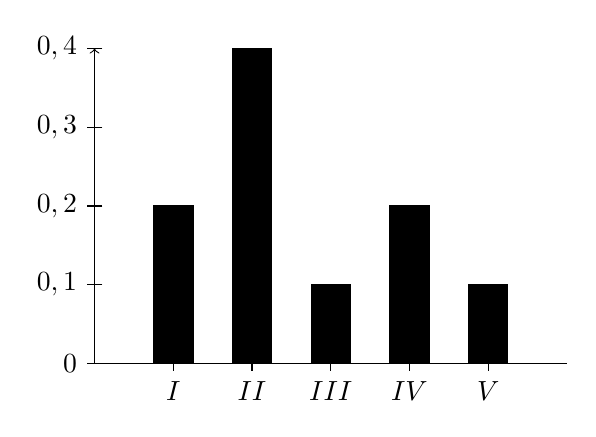
\begin{tikzpicture}
                \draw (0,0) -- (6,0);
                \draw[->] (0,0) -- (0,4);
                \draw (1,.1) -- (1,-.1) node[below] {\(I\)};
                \draw (2,.1) -- (2,-.1) node[below] {\(II\)};
                \draw (3,.1) -- (3,-.1) node[below] {\(III\)};
                \draw (4,.1) -- (4,-.1) node[below] {\(IV\)};
                \draw (5,.1) -- (5,-.1) node[below] {\(V\)};
                \draw (.1,0) -- (-.1,0) node[left] {\(0\)};
                \draw (.1,1) -- (-.1,1) node[left] {\(0,1\)};
                \draw (.1,2) -- (-.1,2) node[left] {\(0,2\)};
                \draw (.1,3) -- (-.1,3) node[left] {\(0,3\)};
                \draw (.1,4) -- (-.1,4) node[left] {\(0,4\)};
                \draw[fill=black] (.75,0) rectangle (1.25,2);
                \draw[fill=black] (1.75,0) rectangle (2.25,4);
                \draw[fill=black] (2.75,0) rectangle (3.25,1);
                \draw[fill=black] (3.75,0) rectangle (4.25,2);
                \draw[fill=black] (4.75,0) rectangle (5.25,1);
            \end{tikzpicture}
        \end{center}
    \end{example}

    Lassen sich die Merkmalsausprägungen, deren Häufigkeiten in einem Säulendiagramm dargestellt werden, noch durch ein weiteres Merkmal in einzelne Gruppen einteilen, so kann diese zusätzliche Information in das Diagramm aufgenommen werden.
    Hierzu stehen gestapelte und gruppierte Diagramme zur Verfügung.
    Durch eine Vertauschung beider Achsen im Säulendiagramm entsteht ein Balkendiagramm.
    In einem Balkendiagramm sind die unterschiedlichen Beobachtungswerte der Urliste auf der vertikalen Achse und die Häufigkeiten auf der horizontalen Achse abgetragen.

    In einem Kreisdiagramm werden den einzelnen Häufigkeiten eines Datensatzes in einem Kreis Flächen in Form von Kreissegmenten zugeordnet, wobei die Größe der Fläche proportional zur relativen Häufigkeit gewählt wird.
    Der Winkel eines Kreissegmentes (und damit die Größe des Segmentes) lässt sich als Produkt aus der entsprechenden relativen Häufigkeit und der Winkelsumme im Kreis, d.h. \(360^\circ\), berechnen.
    Da die Summe der relativen Häufigkeiten eins ergibt, wird auf diese Weise die gesamte Kreisfläche abgedeckt.
    Neben oder in den Kreissegmenten (bzw. in einer Legende) wird vermerkt, auf welche Merkmalsausprägungen sich diese beziehen.
    \begin{center}
        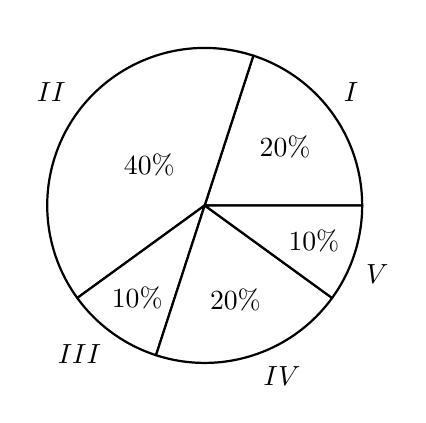
\begin{tikzpicture}
            \pie[radius=2,color={white,white,white,white,white}] {20/\(I\),40/\(II\),10/\(III\),20/\(IV\),10/\(V\)};
        \end{tikzpicture}
    \end{center}

    Eine weitere Möglichkeit der graphischen Aufbereitung von Daten bietet das Liniendiagramm.
    Wird es zur Darstellung von Häufigkeiten verwendet, so ist auch diese Bezeichnung Häufigkeitspolygon anzutreffen.
    Bei dieser Graphik werden die absolute oder die relative Häufigkeit auf der vertikalen Achse eines Koordinatensystems abgetragen, die verschiedenen Merkmalsausprägungen auf der horizontalen Achse.
    Die konkret beobachteten Häufigkeiten werden als Punkte in das Diagramm eingetragen und dann -- zur besseren Veranschaulichung -- durch Linien miteinander verbunden.
    \begin{center}
        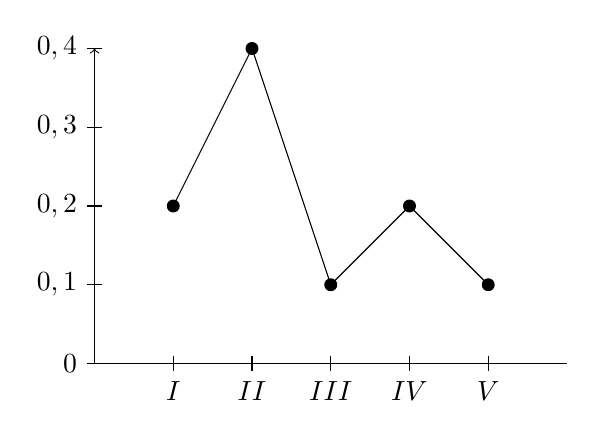
\begin{tikzpicture}
            \draw (0,0) -- (6,0);
            \draw[->] (0,0) -- (0,4);
            \draw (1,.1) -- (1,-.1) node[below] {\(I\)};
            \draw (2,.1) -- (2,-.1) node[below] {\(II\)};
            \draw (3,.1) -- (3,-.1) node[below] {\(III\)};
            \draw (4,.1) -- (4,-.1) node[below] {\(IV\)};
            \draw (5,.1) -- (5,-.1) node[below] {\(V\)};
            \draw (.1,0) -- (-.1,0) node[left] {\(0\)};
            \draw (.1,1) -- (-.1,1) node[left] {\(0,1\)};
            \draw (.1,2) -- (-.1,2) node[left] {\(0,2\)};
            \draw (.1,3) -- (-.1,3) node[left] {\(0,3\)};
            \draw (.1,4) -- (-.1,4) node[left] {\(0,4\)};
            \draw[fill=black] (1,2) circle (.75mm);
            \draw[fill=black] (2,4) circle (.75mm);
            \draw[fill=black] (3,1) circle (.75mm);
            \draw[fill=black] (4,2) circle (.75mm);
            \draw[fill=black] (5,1) circle (.75mm);
            \draw (1,2) -- (2,4) -- (3,1) -- (4,2) -- (5,1);
        \end{tikzpicture}
    \end{center}
    Gerade bei Liniendiagrammen sind Irreführungen und Missinterpretationen leicht möglich.
    Ein Liniendiagramm sollte (für einen einzelnen Datensatz) daher nur eingesetzt werden, wenn auf der Abszisse ein ordinales Merkmal abgetragen wird (z.B. die Zeit) und damit eine sinnvolle Anordnung der Ausprägungen vorgegeben ist.
    Liniendiagramme eignen sich beispielsweise zur Darstellung von Umsätzen über die Zeit von Wertpapierkursen (Entwicklung des Kurses einer Aktie an einem Handelstag der Börse).
    In dieser Situation wird das Liniendiagramm auch als Verlaufskurve (Kurvendiagramm) bezeichnet.
    Dieser Diagrammtyp bietet sich daher zur Darstellung von Daten an, die über einen bestimmten Zeitraum beobachtet wurden (z.B. die Entwicklung der Anzahl von Angestellten in einem Unternehmen).

    Durch die Darstellung mehrerer Linien in einem Liniendiagramm ist auch ein Vergleich von gleichartigen Datensätzen möglich.

    Die vorgestellten Diagrammtypen (Stab-, Säulen-, Balken-, Kreis- und Liniendiagramm) können zur Darstellung von Häufigkeiten in einem beliebig skalierten Datensatz verwendet werden.
    Dabei ist jedoch Folgendes zu beachten: Auch wenn prinzipiell beliebige auf nominalem Niveau erhobene Daten mittels dieser Diagramme graphisch aufbereitet werden können, so entstehen doch wenig aussagekräftige Graphiken, wenn sehr viele verschiedene Beobachtungswerte vorliegen (z.B. bei Beobachtung eines stetigen Merkmals).
    Häufigkeiten und deren graphische Darstellung sind daher meist kein adäquates Mittel zur Aufbereitung solcher Daten.
    Andere graphische Hilfsmittel wie z.B. das Histogramm sind für stetige Merkmale besser geeignet.


    \section*{Klassierte Daten und Histogramm}

    Zentraler Aspekt dieses Abschnitts sind Methoden zur (graphischen) Aufbereitung quantitativer Daten, die auf einer Klassifizierung der Urliste beruhen.
    Dies bedeutet, dass die Beobachtungswerte in Klassen zusammengefasst und die resultierenden Daten dann weiterverarbeitet werden.
    Ziel ist es, aussagekräftige Übersichten über die ``Verteilung'' der Daten zu erhalten.


    \section*{Klassenbildung}

    Durch die Zusammenfassung von Daten \(x_1, \ldots, x_n\) in Klassen \(K_1, \ldots, K_M\) entsteht ein Datenmaterial, das als klassiert oder kategorisiert bezeichnet wird.
    Der zugehörige Datensatz heißt klassierter Datensatz.
    Die resultierenden Daten selbst werden als klassiert bezeichnet.
    Wesentlich ist, dass jedes Datum \(x_i\) eindeutig einer Klasse \(K_j\) zugeordnet werden kann.
    Dies bedeutet insbesondere, dass der Schnitt zweier Klassen leer sein muss (d.h. sie sind disjunkt) und dass die Vereinigung aller Klassen den Wertebereich des betrachteten Merkmals überdeckt.
    Im Hinblick auf die hier vorgestellten graphischen Methoden werden nur Intervalle als Klassen betrachtet, obwohl der Vorgang der Klassierung natürlich allgemeinere Mengen zulässt.

    Eine Klassierung kann sinnvoll bei der Darstellung von Daten eines quantitativen Merkmals eingesetzt werden.
    Aufgrund der Struktur stetiger Datensätze eignet sie sich besonders zur deren Aufbereitung.
    Eine Strukturierung der Daten erlaubt deren leichtere Analyse und ermöglicht eine aussagekräftige graphische Aufbereitung.
    Zur Umsetzung der Klassierung wird der Bereich, in dem alle Ausprägungen des betrachteten Merkmals zu finden sind, in eine vorgegebene Anzahl \(M\) von Intervallen (Klassen) eingeteilt.
    Die Längen dieser Intervalle werden als Klassenbreiten bezeichnet.
    Jedem Datum wird dann diejenige Klasse zugeordnet, in der es enthalten ist.
    Die auf diese Weise neu konstruierten Daten können als Ausprägungen eines ordinalskalierten Merkmals mit \(M\) möglichen Merkmalsausprägungen (den Klassen) interpretiert werden.
    In vielen Erhebungen sind nur klassierte Daten für gewisse Merkmale verfügbar (z.B. Einkommen).
    Im Allgemeinen werden die Beobachtungswerte als in einem abgeschlossenen Intervall \(\brackets*{a, b}\) liegend angesehen.
    Die Intervalle der einzelnen Klassen werden nach links offen und nach rechts abgeschlossen (also mit Intervallgrenze) gewählt, um das gesamte Intervall abzudecken, d.h. es wird eine Zerlegung des Intervalls \(\brackets*{a, b}\) in \(M\) Teilintervalle
    \[
        K_1 = \brackets*{v_0, v_1}, K_2 = \left(v_1, v_2\right], \ldots, K_M = \left(v_{M - 1}, v_M\right]
    \]
    mit \(a = v_0\) und \(b = v_M\) vorgenommen.
    \begin{center}
        \begin{tikzpicture}
            \draw (1.5,.25) -- (1.5,-.25) node[below] {\(a = v_0\)};
            \draw (3,.25) -- (3,-.25) node[below] {\(v_1\)};
            \draw (3.5,.25) -- (3.5,-.25) node[below] {\(v_2\)};
            \draw (5.5,.25) -- (5.5,-.25) node[below] {\(v_3\)};
            \draw (7,.25) -- (7,-.25) node[below] {\(\cdots\)};
            \draw (10,.25) -- (10,-.25) node[below] {\(\cdots\)};
            \draw (12,.25) -- (12,-.25) node[below] {\(v_{M - 1}\)};
            \draw (14,.25) -- (14,-.25) node[below] {\(v_M = b\)};
            \draw[->] (1,0) -- (14.5,0);
        \end{tikzpicture}
    \end{center}
    Die erste Klasse nimmt eine besondere Rolle ein, das entsprechende Intervall ist nämlich sowohl nach rechts als auch nach links abgeschlossen.
    Die Differenzen \(b_j = v_j - v_{j - 1}, j \in \braces*{1, \ldots, M}\), sind die jeweiligen Klassenbreiten.

    \begin{definition}
        Eine Einteilung des Wertebereichs \(\brackets*{a, b}\) in Intervalle
        \[
            K_1 = \brackets*{v_0, v_1}, K_2 = \left(v_1, v_2\right], \ldots, K_M = \left(v_{M - 1}, v_M\right]
        \]
        mit \(a = v_0 < v_1 < \cdots < v_{M - 1} < v_M = b\) heißt \emph{Zerlegung} von \(\brackets*{a, b}\).
    \end{definition}

    Manchmal ist es zweckmäßig, unbeschränkte Intervalle zu betrachten.
    Kann z.B. ein Merkmal (theoretisch) unbeschränkt große Werte (Jahresumsatz, monatliches Einkommen, etc.) annehmen, so ist es sinnvoll, das Intervall der letzten Klasse als nach oben unbeschränkt, d.h. als ein Intervall der Form \(K_M = \parentheses*{v_{M - 1}, \infty}\), zu definieren.
    Analog sind auch Fälle denkbar, in denen die erste Klasse nicht nach unten beschränkt ist und dementsprechend \(K_1 = \left(-\infty, v_1\right]\) gewählt wird.
    Klassen, die zu solchen nicht beschränkten Intervallen gehören, werden als offene Klassen bezeichnet.

    Für klassierte Daten werden absolute Häufigkeiten der einzelnen Klassen durch Summierung der absoluten Häufigkeiten aller verschiedenen Merkmalsausprägungen, die in der jeweiligen Klasse enthalten sind, gebildet. Die relativen Häufigkeiten der Klassen ergeben sich analog als Summe der entsprechenden relativen Einzelhäufigkeiten.

    \begin{definition}
        Der Datensatz \(x_1, \ldots, x_n \in \brackets*{a, b}\) habe die verschiedenen Merkmalsausprägungen \(u_1, \ldots, u_m\) mit absoluten Häufigkeiten \(n_1, \ldots, n_m\) und relativen Häufigkeiten \(f_1, \ldots, f_m\).

        Die \emph{absoluten Häufigkeiten} der Zerlegung \(K_1, \ldots, K_M\) von \(\brackets*{a, b}\) in Klassen sind definiert als
        \[
            n\parentheses*{K_j} = \sum_{u_k \in K_j, k \in \braces*{1, \ldots, m}}n_k, \quad j \in \braces*{1, \ldots, M}.
        \]
        Die \emph{relativen Häufigkeiten} der Klassen \(K_1, \ldots, K_M\) sind definiert als
        \[
            f\parentheses*{K_j} = \frac{n\parentheses*{K_j}}{n} = \sum_{u_k \in K_j, k \in \braces*{1, \ldots, m}}f_k, \quad j \in \braces*{1, \ldots, M}.
        \]
    \end{definition}

    Wie bei gewöhnlichen absoluten und relativen Häufigkeiten addieren sich auch bei klassierten Daten die absoluten Häufigkeiten zur Anzahl \(n\) aller Beobachtungen; die Summe der relativen Häufigkeiten ergibt eins:
    \[
        \sum_{j = 1}^M n\parentheses*{K_j} = n, \quad \sum_{j = 1}^M f\parentheses*{K_j} = 1.
    \]
    Für \(j = 1\) gilt unter Verwendung der Indikatorfunktion
    \[
        n\parentheses*{K_1} = \sum_{i = 1}^n \mathbb{I}_{\brackets*{v_0, v_1}}\parentheses*{x_i}
    \]
    und für jedes \(j \in \braces*{2, \ldots, M}\)
    \[
        n\parentheses*{K_j} = \sum_{i = 1}^n \mathbb{I}_{\brackets*{v_{j - 1}, v_j}}\parentheses*{x_i}
    \]
    Eine Häufigkeitsverteilung für klassierte Daten wird analog zum entsprechenden Begriff für die Beobachtungen der Urliste eingeführt, d.h. die Häufigkeitsverteilung eines klassierten Datensatzes ist die Auflistung der relativen Häufigkeiten der aufgetretenen Klassen.
    Die Häufigkeitsverteilung gibt darüber Aufschluss, wie die Merkmalsausprägungen bezogen auf die gewählte Klasseneinteilung im Datensatz verteilt sind.


    \section*{Histogramm}

    In Datensätzen ist es möglich, dass sehr viele verschiedene Beobachtungswerte vorliegen.
    Bei der Messung eines stetigen Merkmals ist es beispielsweise nicht ungewöhnlich, dass alle Beobachtungswerte verschieden sind.
    Für eine graphische Darstellung solcher Daten sind Diagramme, die auf der Häufigkeitsverteilung der Beobachtungswerte \(x_1, \ldots, x_n\) basieren (wie z.B. Stab- oder Säulendiagramme), in der Regel ungeeignet.
    Die Häufigkeitstabelle führt in diesem Fall nicht zu einer komprimierten und damit übersichtlicheren Darstellung der Daten.
    Einen Ausweg aus dieser Problematik bildet die Klassierung solcher Daten.
    Hierbei werden (unter Inkaufnahme eines gewissen Informationsverlusts) die Merkmalsausprägungen in Klassen zusammengefasst. Die Häufigkeiten der einzelnen Klassen können dann für eine graphische Darstellung herangezogen werden.
    Für Klassierungen des Wertebereichs in Intervalle steht das Histogramm als graphisches Hilfsmittel zur Verfügung.
    Im Folgenden wird eine Zerlegung des Wertebereichs in Intervalle vorgenommen, wobei die erste und letzte Klasse keine offenen Klassen sein dürfen.
    Die Klassen seien durch die Intervalle
    \[
        K_1 = \brackets*{v_0, v_1}, K_2 = \left(v_1, v_2\right], \ldots, K_M = \left(v_{M - 1}, v_M\right],
    \]
    deren Klassenbreiten durch \(b_1 = v_1 - v_0, \ldots, b_M = v_M - v_{M - 1}\) und deren relative Klassenhäufigkeiten durch \(f\parentheses*{K_1}, \ldots, f\parentheses*{K_M}\) gegeben.

    \begin{definition}
        Ein Diagramm wird als \emph{Histogramm} bezeichnet, wenn es auf folgende Weise konstruiert wird: Auf einer horizontalen Achse werden die Klassengrenzen \(v_0, \ldots, v_M\) der Intervalle abgetragen.
        Über jedem Intervall \(K_j\) wird ein Rechteck gezeichnet, dessen Breite gleich der Länge des Intervalls, also der Klassenbreite \(b_j\), ist.
        Die Höhe \(h_j\) des Rechtecks berechnet sich gemäß der Formel
        \[
            h_j = \frac{\text{relative Häufigkeit der zum Intervall gehörigen Klasse}}{\text{Länge des Intervalls}} = \frac{f\parentheses*{K_j}}{b_j}.
        \]
    \end{definition}

    Graphisch ist das Konstruktionsprinzip der Histogrammsäulen in der folgenden Abbildung dargestellt.
    \begin{center}
        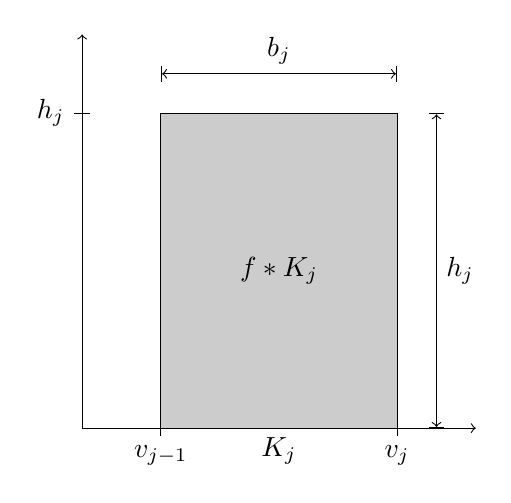
\begin{tikzpicture}
            \draw[->] (0,0) -- (5,0);
            \draw[->] (0,0) -- (0,5);
            \draw[fill=white!80!black] (1,0) rectangle (4,4) node[pos=.5] {\(f\parentheses*{K_j}\)};
            \draw (1,0) -- (1,-.1) node[below] {\(v_{j - 1}\)};
            \draw (4,0) -- (4,-.1) node[below] {\(v_{j}\)};
            \draw (.1,4) -- (-.1,4) node[left] {\(h_j\)};
            \draw[|<->|] (1,4.5) -- (4,4.5) node[midway,above] {\(b_j\)};
            \draw[|<->|] (4.5,0) -- (4.5,4) node[midway,right] {\(h_j\)};
            \node[anchor=north] at (2.5,0) {\(K_j\)};
        \end{tikzpicture}
    \end{center}
    In einem derart konstruierten Histogramm ist der Flächeninhalt eines Rechtecks gleich der relativen Häufigkeit der zugehörigen Klasse:
    \[
        \text{Flächeninhalt des Rechtecks der Klasse }K_j = b_j \cdot h_j = f\parentheses*{K_j}.
    \]
    Aus Gründen der Darstellung kann ein Proportionalitätsfaktor \(c > 0\) eingeführt werden, der etwa eine Skalierung der Achsen ermöglicht.
    Unter Verwendung eines Proportionalitätsfaktors sind die Flächeninhalte der Rechtecke proportional zu den relativen Häufigkeiten der Klassen, d.h.
    \[
        \text{Flächeninhalt des Rechtecks der Klasse }K_j = c \cdot b_j \cdot h_j = cf\parentheses*{K_j}.
    \]
    Dies ist beispielsweise dann der Fall, wenn an Stelle der relativen Klassenhäufigkeiten \(f\parentheses*{K_j}\) in der Definition der Höhen der Rechtecke die absoluten Klassenhäufigkeiten \(n\parentheses*{K_j}\) verwendet werden (Proportionalitätsfaktor \(c = n\)).

    Das Histogramm ist ein Flächendiagramm, d.h. die zu visualisierenden Größen (in diesem Fall die Häufigkeiten) werden im Diagramm proportional zu einer Fläche dargestellt.
    Hierdurch unterscheidet sich das Histogramm von Diagrammformen wie dem Stab- oder Säulendiagramm, in denen die relevanten Informationen durch Höhen beschrieben werden.
    Da in Säulendiagrammen alle Säulen die selbe Breite haben, sind sowohl die Höhen als auch die Flächen der Säulen proportional zur relativen Häufigkeit.
\end{document}
